\documentclass[]{article}
\usepackage{graphicx}
\usepackage{float}
\usepackage{listings}
\usepackage{tipa}
%opening
\title{Assignment \#1: XFST}
\author{Thuong-Hai Pham}

\begin{document}

\maketitle

\begin{abstract}

\end{abstract}

\section{Task 1}
A regular expression (in xfst) allows us to look up \{"sang", "sung"\} and get "sing" should be:

\begin{lstlisting}
[s i n g .x. s [a | u] n g]
\end{lstlisting}

and its corresponding FST:

\begin{figure}[h]
	\centering
	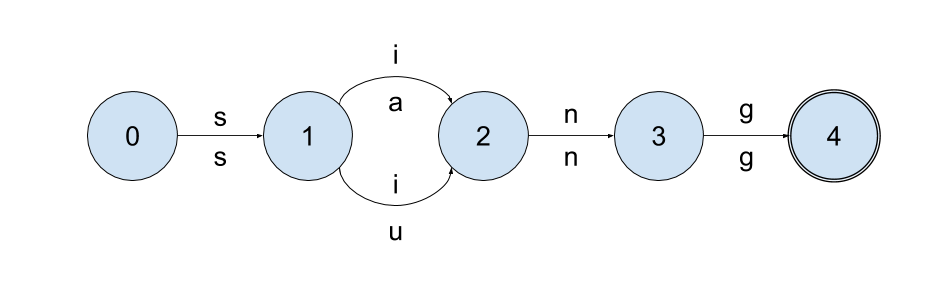
\includegraphics[scale=0.4]{xfst-task1}
	\caption{Task 1 - FST}
	\label{fig:xfst-task1}
\end{figure}

\section{Task 2}

For the requested behavior, our FST diagram should be:

\begin{figure}[H]
	\centering
	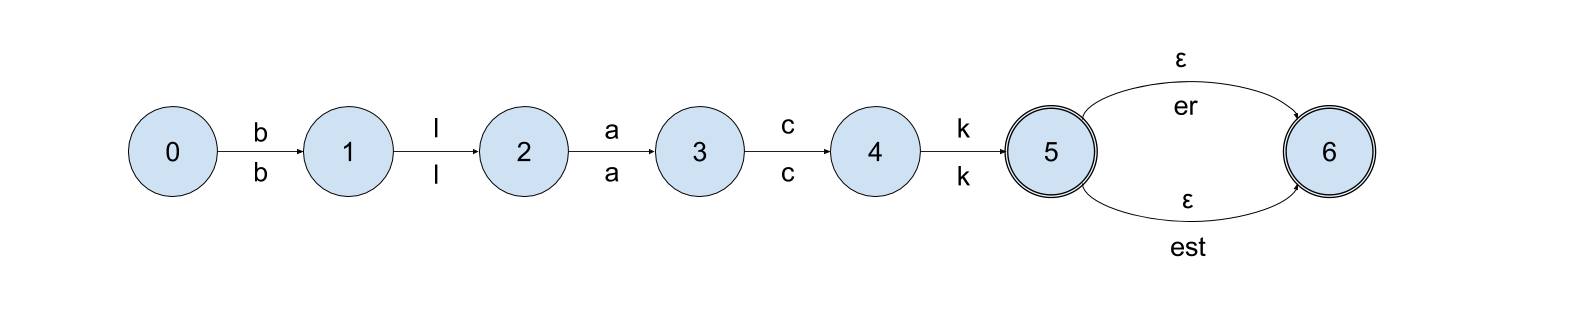
\includegraphics[scale=0.27]{xfst-task2}
	\caption{Task 2 - FST}
	\label{fig:xfst-task2}
\end{figure}


Having that design, our "define" command will be:

\begin{lstlisting}
define task2 [b l a c k [0 .x. [0 | er | est]]]
\end{lstlisting}

\section{Task 3}
To add "green" to the network, we define the following expression:

\begin{lstlisting}
define task3 [[b l a c k | g r e e n] [0 .x. [0 | er | est]]]
\end{lstlisting}


\begin{figure}[H]
	\centering
	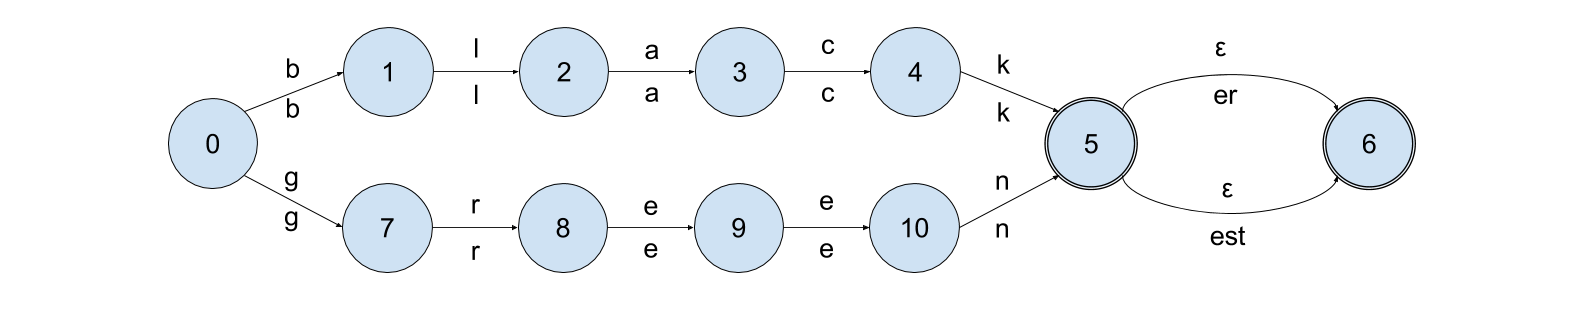
\includegraphics[scale=0.27]{xfst-task3}
	\caption{Task 3 - FST}
	\label{fig:xfst-task3}
\end{figure}

\section{Task 4}

\begin{lstlisting}
define adjs [b l a c k | g r e e n];
define suf [[%+ADJ .x. 0] [0 | [%+CMP .x. er] | [%+SUP .x. est]]];
define task4 [adjs suf];
\end{lstlisting}


\begin{figure}[H]
	\centering
	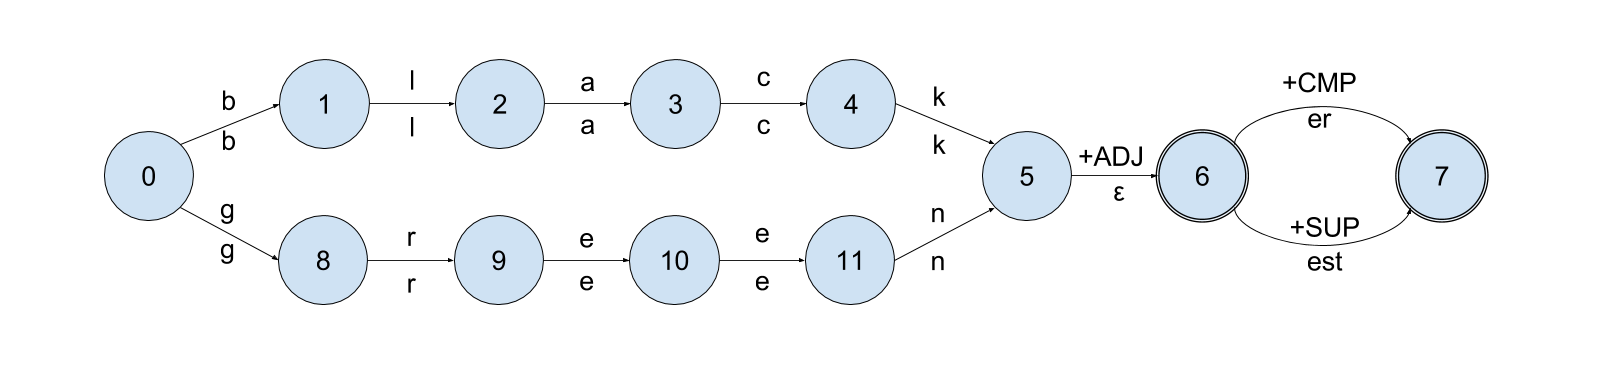
\includegraphics[scale=0.27]{xfst-task4}
	\caption{Task 4 - FST}
	\label{fig:xfst-task4}
\end{figure}


\section{Task 5}
If we add "blue" to the network in figure \ref{fig:xfst-task4} as in the way we add "green", the output of "down blue+ADJ+CMP" will be "blueer" instead of "bluer". The problem occurs because "blue" ends with an "e".

\section{Task 6}

Since we can not add "blue" and its similar adjectives to adjs list in task 4, we have to use two-layer architecture. One layer handles the lexical to intermediate, and one from intermediate to surface words, which handles the spelling variation (remove duplicated e in "blueer").

\begin{figure}[H]
	\centering
	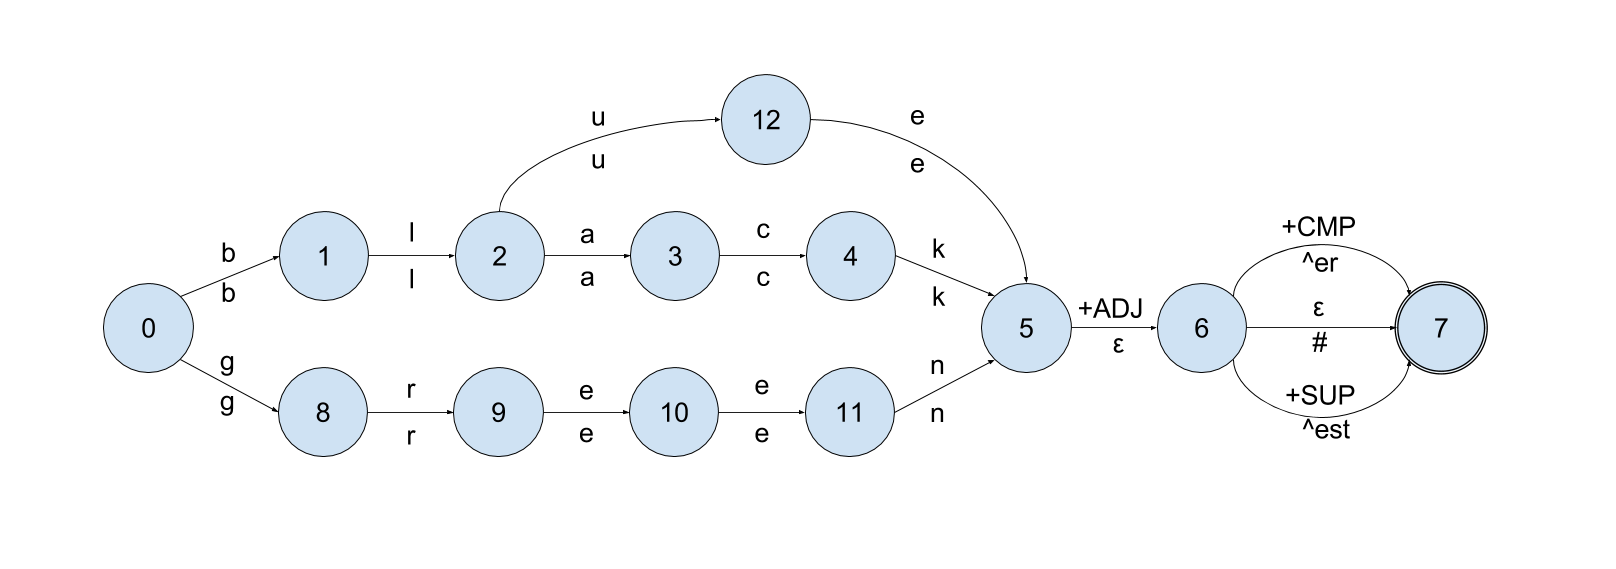
\includegraphics[scale=0.27]{xfst-task6a}
	\caption{Task 6 - Lexical-Intermediate FST}
	\label{fig:xfst-task6a}
\end{figure}

\begin{lstlisting}
define adj [{black} | {green} | {blue}];
define suf [[%+ADJ .x. 0] [0 | [%+CMP .x. [%^ er]] | [%+SUP .x. [%^ est]]]];
define task6a [adj suf];
\end{lstlisting}

\begin{figure}[H]
	\centering
	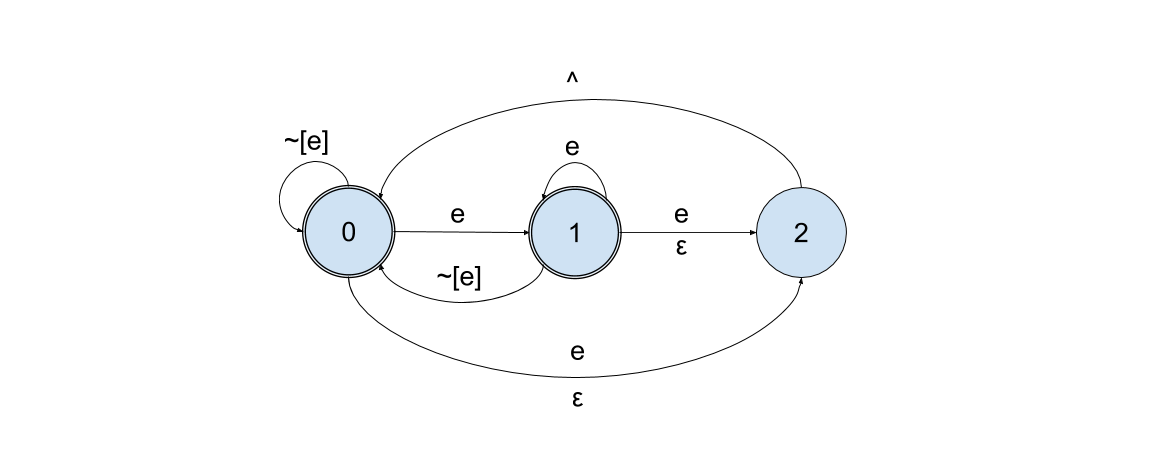
\includegraphics[scale=0.27]{xfst-task6b}
	\caption{Task 6 - e-deletion rule FST}
	\label{fig:xfst-task6b}
\end{figure}

\begin{lstlisting}
define task6b e -> 0 || _ %^;
define task6 task6a .o. task6b .o. [%^ -> 0];
\end{lstlisting}

\section{Task 7}
The word "hot" has its comparative and superlative forms as "hotter" and "hottest",respectively. The letter "t" is doubled before "er" and "est". This also happens to adjectives with short sound of a vowel: \textipa{/\ae/, /e/, /I/, /6/, /2/}. Or on the word surface, these words have one syllable and end with a pair of one vowel, one consonant (except c, q, w, x and y). Ex: (wet, wetter, wettest), (big, bigger, biggest), (sad, sadder, saddest), (thin, thinner, thinnest)\dots


\begin{lstlisting}
define C [b|c|d|f|g|h|j|k|l|m|n|p|q|r|s|t|v|w|x|y|z];
define V [a|e|i|o|u];
define Ca [C - [c|q|w|x|y]];
define REP {^2};

define adj [{black} | {green} | {blue} | {hot} | {thin}];

define suf [[%+ADJ .x. 0] [0 | [%+CMP .x. [%- er]] | [%+SUP .x. [%- est]]]];

define task6b e -> 0 || _ %-;

define task7b Ca -> "[" ... "]" REP || 0 C+ V _ %-;

define rmminus %- -> 0;

define task7 0:"^[" [[adj suf] .o. task6b .o. task7b .o. rmminus] 0:"^]";

regex task7;

set retokenize off

compile-replace lower

down blue+ADJ+CMP
down green+ADJ+CMP
down hot+ADJ+CMP

lower
\end{lstlisting}

In the code snippet above, we use "-" to separate each morpheme instead of "\^{}" as in task 6 because "\^{}" is duplication operator. The lower words after "regex task7":

\begin{lstlisting}
^[thin^]
^[thi[n]^2er^]
^[thi[n]^2est^]
^[hot^]
^[ho[t]^2er^]
^[ho[t]^2est^]
^[greener^]
^[greenest^]
^[green^]
^[blue^]
^[bluer^]
^[bluest^]
^[blacker^]
^[blackest^]
^[black^]
\end{lstlisting}

Then, we make use of the duplication operator in compile-replace command to produce the desired outputs.

\begin{lstlisting}
thin
thinnest
thinner
hot
hottest
hotter
green
greener
greenest
blue
bluer
bluest
black
blacker
blackest
\end{lstlisting}

\section{Task 8}
For irregular adjective like "good", we compile them as special cases:
\begin{lstlisting}
define adjgood [[g o o d [%+ADJ .x. 0]] |
	[[g o o d %+ADJ %+CMP] .x. {better}] |
	[[g o o d %+ADJ %+SUP] .x. {best}]]
\end{lstlisting}

\end{document}
